%versi 2 (8-10-2016)
\chapter{Landasan Teori}
\label{chap:teori}


 
Pada bab ini akan dibahas mengenai dasar teori yang digunakan pada penyusunan tugas akhir. Pembahasan pertama mencakup hal-hal yang berkaitan dengan pengertian kewirausahaan dari umum sampai khusus yaitu kewirausahaan menurut GEM. Pembahasan kedua yaitu tentang teori dan aplikasi dari CA (Cellular Automata) khususnya tentang ECA (Entrepreneur Cellular Automata). Pembahasan terakhir tentang hal-hal lain yang mendukung implementasi perangkat lunak seperti bahasa pemrograman java.


\section{Arti Kewirausahaan}
\label{sec:artiwirausaha}

\graphicspath{{images/}}

Secara umum arti kewirausahaan merupakan suatu proses dalam mengerjakan sesuatu yang baru dan berbeda yang bermanfaat bagi orang lain atau diri sendiri. Orang yang melakukan proses kewirausahaan adalah wirausaha. Ciri-ciri wirausaha antara lain yaitu berani mengambil risiko, memiliki semangat dan kemauan keras, memiliki jiwa pemimpin, dsb. Tujuan wirausaha sendiri yaitu menciptakan lapangan kerja yang baru dan meningkatkan jumlah para wirausaha di suatu negara.


Kewirausahaan menurut GEM merupakan proses yang terdiri dari fase-fase berbeda mulai dari niat mendirikan suatu usaha, menjalankan suatu usaha baru atau sudah berdiri, sampai dengan penghentian sebuah usaha. Proses ini dimulai dengan keterlibatan individu yang berpotensi untuk menjadi wirausaha, yaitu mereka yang percaya bahwa mereka mempunyai kemampuan untuk memulai suatu usaha, individu yang melihat kesempatan untuk berwirausaha dan individu yang tidak takut gagal dalam memulai suatu usaha.


GEM melakukan penelitiannya dengan didasarkan pada premis-premis berikut. Pertama, kemakmuran sebuah ekonomi sangat tergantung pada sektor kewirausahaan yang dinamis. Sifat dari kegiatan ini dapat beragam karakter dan dampaknya. Kewirausahaan yang didorong oleh kebutuhan khususnya di wilayah yang kurang berkembang atau wilayah yang sedang mengalami penurunan lapangan kerja, dapat membantu ekonomi suatu negara jika memang lapangan pekerjaan terbatas. Di sisi lain, pada wilayah yang lebih berkembang kesempatan wirausaha terjadi lebih akibat dari kemakmuran dan kemampuan inovasi mereka. Kedua, kapasitas kewirausahaan sebuah ekonomi didasarkan pada kemampuan dan motivasi individunya untuk memulai suatu usaha dan dapat diperkuat oleh persepsi positif masyarakat tentang kewirausahaan. Terakhir, pertumbuhan tinggi kewirausahaan adalah kontributor utama untuk penyedia lapangan pekerjaan dan persaingan antar negara bergantung pada usaha yang inovatif.
\begin{figure} 
	\centering  
	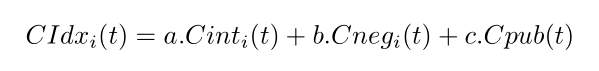
\includegraphics[width=14cm, height=6cm]{Capture}  
	\caption[Fase Wirausaha]{Fase Wirausaha} 
	\label{fig:artiwirausaha} 
\end{figure}

Pada gambar \ref{fig:artiwirausaha}, dijelaskan fase pertama dari ilustrasi GEM adalah wirausaha \textit{nascent}. Wirausaha \textit{nascent} adalah mereka yang telah memulai suatu usaha baru namun masih sangat dini (< 3 bulan). Setelah lebih dari tiga bulan, wirausaha \textit{nascent} ini disebut Pemilik Usaha Baru (\textit{new business owner}). Fase ini dijalani sampai individu tersebut telah tiga setengah tahun tahun terlibat dalam kewirausahaan. Kegiatan pada fase wirausaha \textit{nascent} dan pemilik usaha baru masuk kedalam kelompok Total Early Stage Entrepreneurial Activity (TEA). Fase selanjutnya adalah fase dimana wirausaha disebut sebagai Pemilik Usaha Mapan (\textit{owner-manager of an established business}). 

GEM mempertimbangkan beberapa indikator yang mempengaruhi berlangsungnya kewirausahaan di suatu negara yaitu \textit{Entrepreneurial Intention}, \textit{Fear of Failure}, \textit{perceived opportunities} dan \textit{Perceived Capabilities}. \textit{Entrepreneurial Intention} mendeskripsikan populasi yang bertekad untuk mendirikan suatu usaha dalam waktu tiga tahun kedepan. \textit{Fear of Failure} mendeskripsikan populasi yang positif yang mengindikasikan bahwa takutnya gagal dalam menghambat mereka dalam mendirikan suatu usaha. \textit{Perceived Opportunities} mendeskripsikan populasi yang melihat kesempatan bagus untuk memulai suatu usaha di daerah tempat tinggal mereka. \textit{Perceived Capabilities} mendeskripsikan populasi yang merasa mempunyai kemampuan dan pengetahuan yang cukup untuk mendirikan suatu usaha.

GEM melihat penduduk yang berpotensi menjadi wirausaha di Indonesia
dilihat dari tiga indikator yaitu \textit{perceived opportunities}, \textit{perceived capabilities} dan \textit{role model}. \textit{Perceived Opportunities} mengukur persentase dari orang dewasa antara usia 18 sampai 64 tahun yang melihat kesempatan bagus untuk memulai usaha di tempat mereka tinggal. Seperti pada gambar \ref{fig:perceivedopportunity}, diantara semuanya yang melihat adanya kesempatan baik untuk memulai usaha baru, pria muda (antara 25 sampai 34 tahun) memiliki perceived opportunities lebih tinggi dari wanita yang seusianya. Namun, untuk wanita diatas usia 35 tahun melihat adanya kesempatan lebih tinggi dari pria pada kelompok usia yang sama.

\begin{figure} [H]
	\centering  
	\includegraphics[width=14cm, height=6cm]{POumur} 
	\caption[Komposisi perceived opportunity untuk kelompok usia yang berbeda]{Komposisi perceived opportunity untuk kelompok usia yang berbeda} 
	\label{fig:perceivedopportunity} 
\end{figure}

Menurut data GEM, orang dewasa yang berpendidikan sekolah menengah atas memiliki perceived opportunities paling tinggi di antara orang dewasa Indonesia. Ketika mereka menjalani pendidikan di universitas untuk pendidikan yang lebih tinggi, perceived opportunities mereka cenderung menurun (Lihat Gambar \ref{fig:POPendidikan}). Umumnya Jakarta memiliki persepsi yang lebih tinggi tentang perceived opportunities, diikuti kota Bandung, Surabaya, Semarang dan Surakarta. Kota-kota tersebut terletak di pulau Jawa dimana aktivitas ekonomi terkonsentrasi di sana. Kota yang terletak di pulau lain cenderung menerima persepsi adanya kesempatan yang lebih rendah (< 1\%) adalah Banda Aceh dan Pontianak (Lihat Gambar \ref{fig:POdomisili}). Berdasarkan tingkat pendapatan dan berdasarkan jenis kelamin, tidak ada perbedaan jenis kelamin pada perceived opportunities antara tingkat pendapatan. Terdapat 83,8\% dan 84,2\% wanita dengan pendapatan per bulan dibawah 5 juta rupiah yang mempertimbangkan adanya kesempatan yang baik untuk memulai usaha (Lihat Gambar \ref{fig:POpendapatan}).

\begin{figure} [H]
	\centering  
	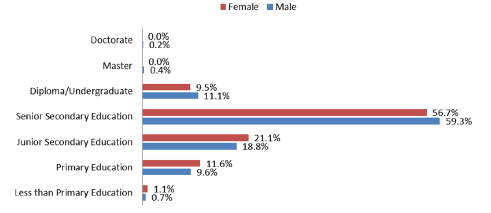
\includegraphics[width=14cm, height=6cm]{POPendidikan} 
	\caption[Komposisi perceived opportunity untuk tingkat pendidikan yang berbeda] {Komposisi perceived opportunity untuk tingkat pendidikan yang berbeda} 
	\label{fig:POpendidikan} 
\end{figure}

\begin{figure} [H]
	\centering  
	\includegraphics[width=15cm, height=10cm]{POdomisili} 
	\caption[Komposisi perceived opportunity berdasarkan domisili]{Komposisi perceived opportunity berdasarkan domisili} 
	\label{fig:POdomisili} 
\end{figure}

\begin{figure} [H]
	\centering  
	\includegraphics[width=14cm, height=7cm]{POpendapatan} 
	\caption[Komposisi perceived opportunity berdasarkan pendapatan]{Komposisi perceived opportunity berdasarkan pendapatan} 
	\label{fig:POpendapatan} 
\end{figure}

Indikator kedua yang mempengaruhi keberlangsungan wirausaha yaitu Perceived Capabilities. Perceived Capabilities mencerminkan persentase orang dewasa berusia antara 18 dan 64 tahun yang percaya mereka memiliki keterampilan, pengetahuan dan pengalaman yang diperlukan untuk memulai usaha baru. Gambar \ref{fig:PCumur} menunjukkan berdasarkan pengelompokan usia, individu antara 25 dan 34 tahun merasa bahwa mereka memiliki kemampuan untuk memulai sebuah usaha baru lebih tinggi dari golongan usia lainnya, yang diikuti oleh individu golongan usia 35-44 tahun.

\begin{figure} [ht]
	\centering  
	\includegraphics[width=14cm, height=7cm]{PCumur} 
	\caption[Komposisi perceived capabilities berdasarkan usia]{Komposisi perceived capabilities berdasarkan usia} 
	\label{fig:PCumur} 
\end{figure}

Berdasarkan tingkat pendidikan, mereka yang telah menyelesaikan pendidikan sekolah menengah merasa memiliki kemampuan kewirausahaan yang lebih tinggi (> 50\%) daripada individu yang berpendidikan lebih rendah. Namun, Perceived Capabilities cenderung lebih rendah bagi mereka yang telah menyelesaikan pendidikan di tingkat universitas (Lihat Gambar \ref{fig:PCpendidikan}). Berdasarkan tingkat pendapatan, baik pria maupun wanita memiliki perceived capability tertinggi untuk pendapatan dibawah 5 juta rupiah. Tetapi pada tingkat pendapatan yang lebih tinggi, yaitu diatas 15 juta rupiah, data mengindikasikan bahwa 0,4\% wanita memandang mereka memiliki kemampuan dan pengetahuan untuk memulai usaha baru. Hal ini lebih tinggi dibandingkan pria yang hanya 0,2\% (Lihat Gambar \ref{fig:PCpendapatan}). 

\begin{figure} [H]
	\centering  
	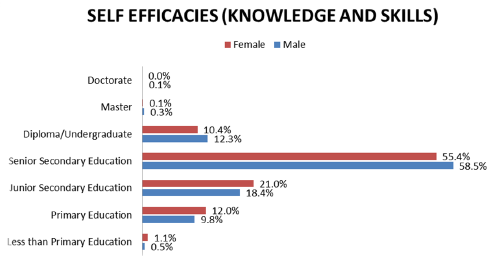
\includegraphics[width=14cm, height=7cm]{PCpendidikan} 
	\caption[Komposisi perceived capabilities berdasarkan tingkat pendidikan]{Komposisi perceived capabilities berdasarkan tingkat pendidikan} 
	\label{fig:PCpendidikan} 
\end{figure}
 

\begin{figure} [ht]
	\centering  
	\includegraphics[width=14cm, height=7cm]{PCpendapatan} 
	\caption[Komposisi perceived capabilities berdasarkan tingkat pendapatan bulanan (dalam juta rupiah)]{Komposisi perceived capabilities berdasarkan tingkat pendapatan bulanan (dalam juta rupiah)} 
	\label{fig:PCpendapatan} 
\end{figure}

Sama seperti Perceived Opportunities, Jakarta memperoleh Perceived Capabilities lebih tinggi dalam orang-orang yang percaya memiliki kemampuan, pengetahuan dan pengalaman untuk memulai usaha baru. Gambar \ref{fig:PCdomisili} menunjukkan perbedaan antar jenis kelamin dalam Perceived Capabilities sangatlah kecil di tiap kota (Perbedaan dibawah 1\%). Hal ini menunjukkan baik pria maupun wanita percaya bahwa mereka memiliki syarat kemampuan untuk ikut dalam kegiatan wirausaha.

\begin{figure} [H]
	\centering  
	\includegraphics[width=14cm, height=10cm]{PCdomisili} 
	\caption[Komposisi perceived capabilities berdasarkan domisili]{Komposisi perceived capabilities berdasarkan domisili} 
	\label{fig:PCdomisili} 
\end{figure}

Indikator terakhir yang mempengaruhi pertumbuhan wirausaha yaitu Role Model. GEM melihat Role Model sebagai ukuran persepsi orang dewasa berusia antara 18 dan 64 tahun yang mengenal seseorang yang memiliki usaha secara personal dalam 2 tahun terakhir. Nilai role model didefinisikan sebagai Know Startup Entrepreneur Rate. Indonesia memiliki tingkat sebesar 67\% dan nilai ini tidak banyak berbeda untuk pria maupun wanita. Seperti ditunjukkan pada Gambar \ref{fig:RMusia}, berdasarkan kategori usia, individu berusia antara 25 dan 34 tahun memiliki persentasi tertinggi dalam memahami Role Model secara personal.


\begin{figure} [H]
	\centering  
	\includegraphics[width=12cm, height=7cm]{RMusia} 
	\caption[Komposisi role model berdasarkan usia]{Komposisi role model berdasarkan usia} 
	\label{fig:RMusia} 
\end{figure}

Berdasarkan perbedaan tingkat pendapatan, Role Model memiliki peran penting untuk individu dengan tingkat pendapatan per bulan dibawah 7 juta rupiah. Hampir 95,4\% pria dan 95,2\% wanita yang memiliki role model. Pada tingkat pendapatan per bulan di atas 15 juta rupiah, wanita lebih mempertimbangkan Role Model, daripada pria (Lihat Gambar \ref{fig:RMpendapatan}).

\begin{figure} [H]
	\centering  
	\includegraphics[width=12cm, height=7cm]{RMpendapatan} 
	\caption[Komposisi role model berdasarkan tingkat pendapatan]{Komposisi role model berdasarkan tingkat pendapatan} 
	\label{fig:RMpendapatan} 
\end{figure}


\section{Cellular Automata}
\label{sec:cellularautomata}

Cellular Automata (CA) merupakan model matematis untuk sistem dimana banyak komponen sederhana bertindak bersama untuk menghasilkan pola perilaku yang rumit.

